% Compile with XeLaTeX, TeXLive 2013 or more recent
\documentclass{beamer}

% Base packages
\usepackage{fontspec}
\usepackage{xunicode}
\usepackage{xltxtra}

\usepackage{amsfonts}
\usepackage{amsmath}
\usepackage{longtable}
\usepackage{csquotes}
\usepackage{standalone}

% Setup fonts
\newfontfamily\russianfont{CMU Serif}
\setromanfont{CMU Serif}
\setsansfont{CMU Sans Serif}
\setmonofont{CMU Typewriter Text}

% Setup Russian hyphenation. NOTE: this declaration *must* come after fontspec's font declarations,
% or a mysterious (but harmless in other respects) error "Improper `at' size (0.0pt), replaced by 10pt." would appear.
\usepackage{polyglossia}
\defaultfontfeatures{Scale=MatchLowercase, Mapping=tex-text}

\setdefaultlanguage[spelling=modern]{russian} % for polyglossia
\setotherlanguage{english} % for polyglossia

% Vector drawings
\usepackage{tikz}
\usetikzlibrary{shapes, calc, arrows, fit, positioning, decorations, patterns, decorations.pathreplacing, chains, snakes}
\usepackage[siunitx]{circuitikz}

\graphicspath{./../../simbook/metoda/pictures/}

% Be able to insert hyperlinks
\usepackage{hyperref}
\hypersetup{colorlinks=true, linkcolor=black, filecolor=black, citecolor=black, urlcolor=blue , pdfauthor=Grigory Rechistov <grigory.rechistov@phystech.edu>, pdftitle=Курс «Программное моделирование вычислительных систем»}
% \usepackage{url}

% Misc optional packages
\usepackage{underscore}
\usepackage{amsthm}

% A new command to mark not done places
\newcommand{\todo}[1][Напиши меня]{{\color{red}TODO\ #1}}

\title{Роль моделирования в разработке программно-аппаратных платформ}
\subtitle{Курс «Программное моделирование вычислительных систем»}
\subject{Курс «Программное моделирование вычислительных систем»}

\author[]{Григорий Речистов \\ \small{\href{mailto:grigory.rechistov@phystech.edu}{grigory.rechistov@phystech.edu}}}
\date{\today}
\pgfdeclareimage[height=0.5cm]{ilab-logo}{../ilab-noletters.png}
\logo{\pgfuseimage{ilab-logo}}

\typeout{Copyright 2015 Grigory Rechistov}

\usetheme{Berlin}
\setbeamertemplate{navigation symbols}{}%remove navigation symbols

\begin{document}

\begin{frame}
    \maketitle
\end{frame}

\begin{frame}
    \tableofcontents
\end{frame}

\section{Сложность вычислительных систем}

\begin{frame}{Сложность вычислительных систем}

\centering
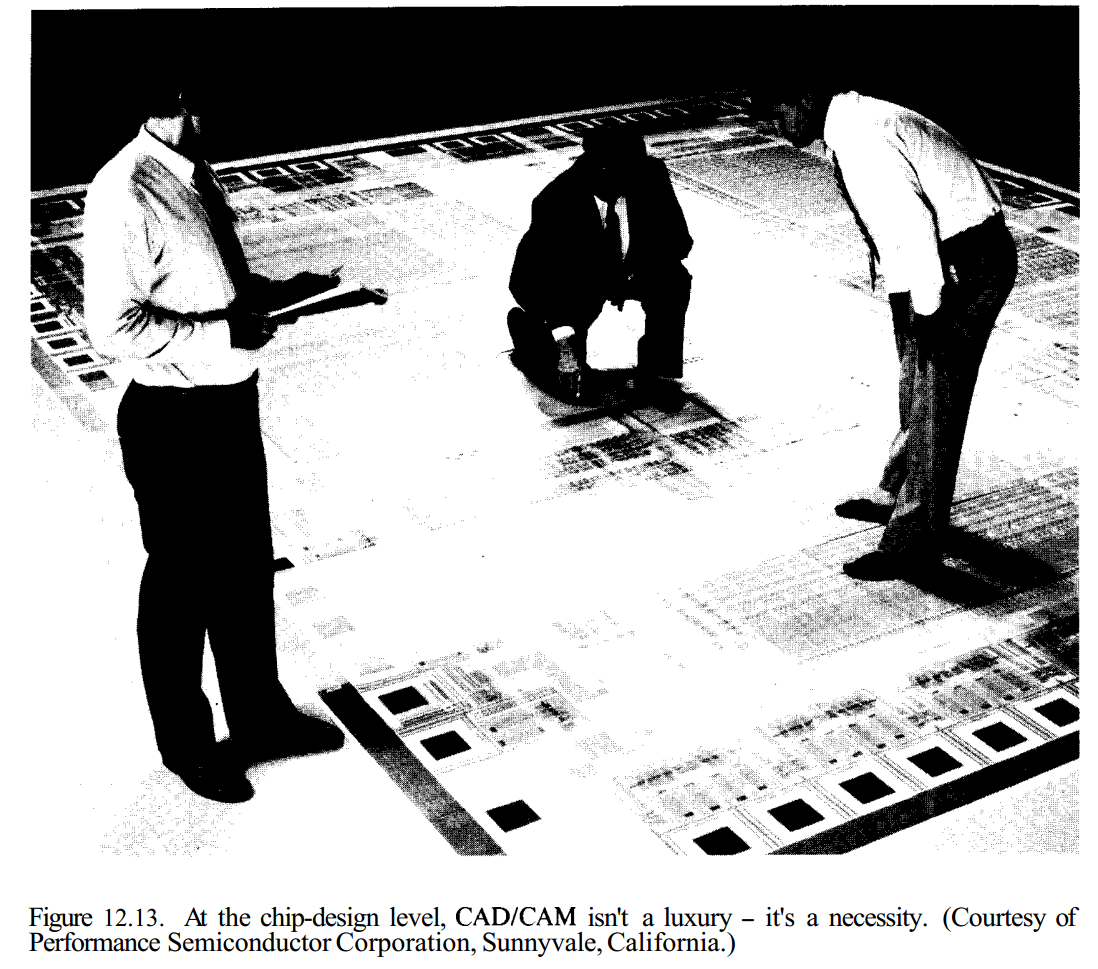
\includegraphics[width=0.7\textwidth]{ic-floor}

\tiny{Иллюстрация из: P. Horowitz and W. Hill. 1989. The Art of Electronics. Cambridge University Press, New York, NY, USA}


\end{frame}

\begin{frame}{Почему разработка только на реальном железе невыгодна }

\begin{itemize}
\item Количество доступных образцов мало
\item Отладка очень сложна
\item Цикл разработки длинный
\end{itemize}

$\Rightarrow$ Стоимость разработки увеличивается

\bigskip

\tiny{I've noticed a shift during the past couple of years towards an increasing use of various types of simulation, including virtual platforms. Previously software developers wanted real hardware, but now they have to start using simulation because there's no chip available. \textit{Tomas Evensen, Wind River CTO}}

\end{frame}

\begin{frame}{Программные модели}
\centering 
\input{./../../simbook/metoda/drawings/idea}

\end{frame}

\section{Области использования моделей}

\begin{frame}{Области использования}

\begin{itemize}
\item Новое аппаратное обеспечение
\item Совместная разработка аппаратуры и программ
\item Экспериментальные архитектуры
\item Предсказание производительности, потребления мощности
\item Обеспечение совместимости с другими архитектурами
\end{itemize}

\end{frame}


\begin{frame}{Новая аппаратура}

\input{./../../simbook/metoda/drawings/error-cost}

\end{frame}

\begin{frame}{Разработка программ и аппаратуры}

\begin{itemize}
\item Firmware, BIOS, UEFI
\item Драйверы устройств
\item Операционные системы
\item Компиляторы
\item Приложения
\end{itemize}

\end{frame}

\begin{frame}{Совместная разработка}

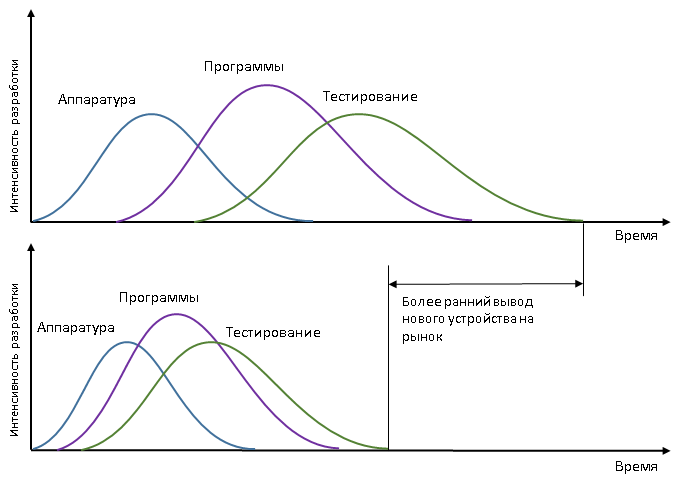
\includegraphics[width=0.8\textwidth]{shift-left} % TODO TikZ-elize this

\end{frame}

\begin{frame}{Экспериментальные архитектуры}

\begin{itemize}
\item Новые ISA
\item Многоядерные системы
\item Векторные системы
\item Безопасность и криптография
\end{itemize}

\end{frame}

\begin{frame}{Предсказание производительности}

\begin{itemize}
\item Untimed
\item Loosely timed
\item Approximately timed
\end{itemize}

\end{frame}


\begin{frame}{Обеспечение совместимости}
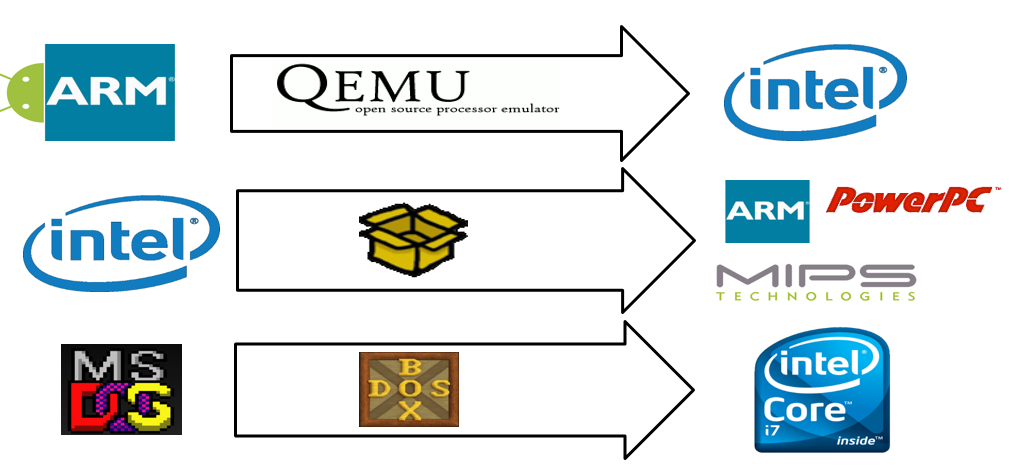
\includegraphics[width=0.8\textwidth]{compat} % TODO TikZ-elize this

\end{frame}

\section{Термины}

\begin{frame}{Терминология}
\begin{itemize}
\item Симуляция — моделирование системы через имитацию внешне видимых эффектов, возникающих при взаимодействии с ней
\item Эмуляция — моделирование системы через имитацию внутренней структуры и процессов, происходящих внутри её подсистем
\item Виртуализация — обеспечение эффективной изоляции нескольких систем друг от друга при одновременном и прозрачном доступе к ресурсам нижележащей системы
\end{itemize}

\end{frame}

\begin{frame}{Типы симуляторов}
\begin{itemize}
\item Полноплатформенные
\item Режима приложения
\item Функциональные
\item Потактовые
\item Программные
\item Гибридные
%\item 
%\item 
\end{itemize}
\end{frame}

\begin{frame}{Терминология}
\begin{itemize}
\item Хозяин, host, инструментальная система
\item Гость, guest, target, целевая система
%\item
%\item
\end{itemize}
\end{frame}

\section{Возможности}

\begin{frame}{Некоторые возможности симуляции}
\begin{itemize}
\item Неразрушающее изучение
\item Повторяемость запусков
\item Сохранение состояния
\item Синхронная остановка
\item Обращение времени
\end{itemize}
\end{frame}

\begin{frame}{Итоги}
\begin{itemize}
\item Программные модели создаются до доступности аппаратуры
\item Они используются повсеместно для совместной разработки программ и железа
\item Симуляция позволяет делать вещи, о которых раньше можно было только мечтать
\end{itemize}
\end{frame}

\begin{frame}{На следующей лекции}
\begin{itemize}
\item Требования на симуляторы
\end{itemize}
\end{frame}


\section{Литература}

\begin{frame}[allowframebreaks]{Литература}
\begin{thebibliography}{99}
    \bibitem{simbook} Программное моделирование вычислительных систем (лекции). \url{http://atakua.doesntexist.org/public/archive/simcourse/simulation-lectures-latest.pdf}

    \bibitem{practicum} Лабораторный практикум по программному моделированию.  \url{http://atakua.doesntexist.org/public/archive/simcourse/simulation-practicum-latest.pdf}

\end{thebibliography}
\end{frame}


% The final "thank you" frame
\begin{frame}

{\huge{Спасибо за внимание!}\par}

\vfill

Слайды и материалы курса доступны по адресу \url{http://is.gd/ivuboc} % http://atakua.doesntexist.org/wordpress/simulation-course-russian/

\vfill

\tiny{\textit{Замечание}: все торговые марки и логотипы, использованные в данном материале, являются собственностью их владельцев. Представленная точка зрения отражает личное мнение автора.
%Материалы доступны по лицензии Creative Commons Attribution-ShareAlike (Атрибуция — С сохранением условий) 4.0 весь мир (в т.ч. Россия и др.). Чтобы ознакомиться с экземпляром этой лицензии, посетите \url{http://creativecommons.org/licenses/by-sa/4.0/}
}

\end{frame}


\end{document}
